
\section{maincontent}

\begin{frame}
\frametitle{Magnetic-Field Effect as a Tool to Investigate 
Electron Correlation in Strong-Field Ionization 
\small (Phys. Rev. Lett. 128, 113201 (2022))}
\framesubtitle{Surrounding concepts}


\small
\begin{textblock*}{200pt}(250pt,60pt)
\begin{itemize}
\item 3 steps model
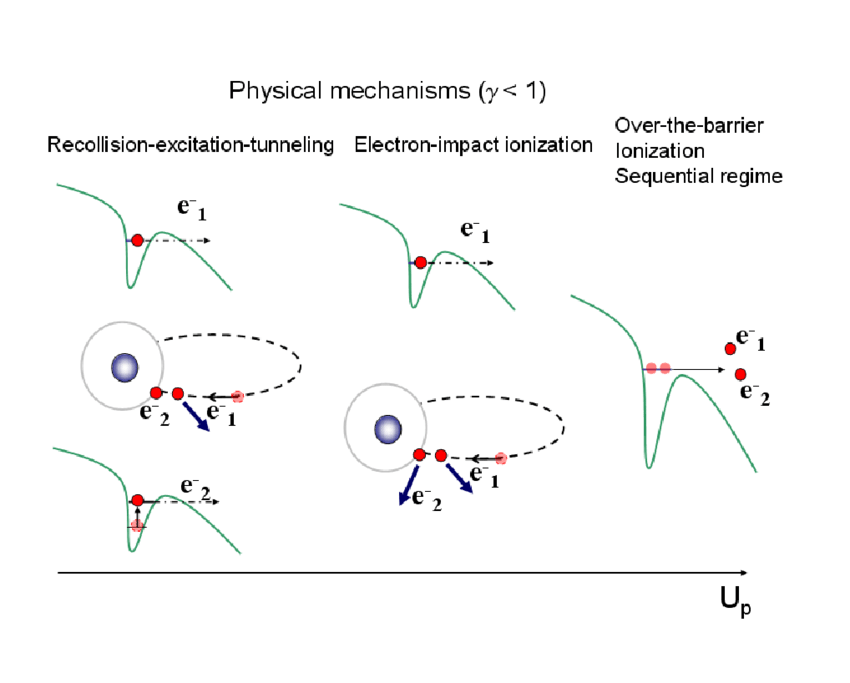
\includegraphics[scale=.20]{images/Color-online-Schematic-representation-of-the-dominant-physical-mechanisms-behind.png}
\end{itemize}
\end{textblock*}

\small
\begin{textblock*}{200pt}(30pt,60pt)
\begin{itemize}
\item Electron correlation
%
\includegraphics[scale=.75]{images/polcls.png}
\begin{align}
\footnotesize
\begin{split}
\Psi(\boldsymbol{r}_1,\boldsymbol{r}_2) \Theta(1,2)
 & = \frac{1}{2}\left[ \varphi_a(\boldsymbol{r}_1)\varphi_b(\boldsymbol{r}_2)
 \pm  \varphi_b(\boldsymbol{r}_1)\varphi_a(\boldsymbol{r}_2) \right] \\
 &\times \left[ \sigma_a(1)\sigma_b(2)
 \pm  \sigma_b(1)\sigma_a(2) \right]
\end{split}
 \nonumber \\
\Psi_H(\boldsymbol{r}_1,\boldsymbol{r}_2) \Theta(1,2)
 & = \varphi_a(\boldsymbol{r}_1)\varphi_b(\boldsymbol{r}_2)
 \sigma_a(1)\sigma_b(2)
 \nonumber
\end{align}
\item Sequential Double Ionization
\item Nonsequential Double Ionization (NSDI)
\begin{itemize}
 \item[$\bullet$] Successfully explained in the dipole approx.
  for a wide range of intensities and wavelengths
 \item[$\bullet$] Can happen a number of different ways
\end{itemize}
%\begin{align}
%\footnotesize
%H = \frac{1}{2}
%\Big( \boldsymbol{p} + q\boldsymbol{A}(x,t) \Big)^2 + V_0, \nonumber \\
%\boldsymbol{A}(x,t) \sim A(t) + \frac{x}{c}F(t) 
%- \frac{1}{2}\frac{x^2}{c^2}\frac{d}{dt}F(t). \nonumber
%\end{align}
%\begin{align}
%\footnotesize
%\boldsymbol{F} = -\frac{\partial \boldsymbol{A}}{\partial t}, \hspace{10pt} 
%\nabla \times \boldsymbol{B} = 
%   \frac{1}{c^2}\frac{\partial\boldsymbol{F}}{\partial t}.
% \nonumber
%\end{align}
\end{itemize}
\end{textblock*}



\begin{textblock*}{100pt}(80pt,210pt)
\begin{align}
\footnotesize
U_p = \frac{F_0^2}{4\omega^2}, \hspace{30pt} 
\gamma = \sqrt{\frac{I_p}{2U_p}}\nonumber
\end{align}
\end{textblock*}

%\begin{textblock*}{400pt}(30pt,130pt)
%\centering\footnotesize
%\begin{align}
%H = \frac{1}{2}
%\Big( \boldsymbol{p} + \boldsymbol{A}(x,t) \Big) \nonumber \\
%\boldsymbol{A}(x,t) \sim A(t) + \frac{x}{c}E(t) 
%- \frac{1}{2}\frac{x^2}{c^2}\frac{d}{dt}E(t) \nonumber
%\end{align}
%
%\end{textblock*}

\end{frame}



\begin{frame}
\frametitle{Magnetic-Field Effect as a Tool to Investigate 
Electron Correlation in Strong-Field Ionization
\small (Phys. Rev. Lett. 128, 113201 (2022))}
\framesubtitle{The state of the problem}

\small
\begin{textblock*}{400pt}(30pt,60pt)
\begin{itemize}
\item In the nondipole case
\item Conservation of momentum for a single electron ionization
\begin{align}
\footnotesize
\left\langle p_{x,e} \right\rangle (E_e)
 = \frac{E_e}{c} + \frac{1}{3}\frac{I_p}{c}. \nonumber
\end{align}
\item Forward shift of $I_p/(3c)$ caused by ionization in itself 
and tunneling through the barrier
\item What about double ionization?
\begin{itemize}
 \footnotesize
 \item[$\bullet$] The naive assumption
 $$ 
   \left\langle p_{x1} + p_{x2} \right\rangle (E_{\rm sum})= 
      \frac{E_{\rm sum}}{c} + \frac{1}{3}\times \frac{I_{p1} + I_{p2}}{c}.
 $$
\end{itemize}
 \item Yes, but what about correlated electrons, as in NDSI? %\footnote{\Tiny Chelkowski \textit{et al.}, Phys. Rev. Lett. 113, 263005, (2014)}
\begin{itemize}
 \footnotesize
 \item[$\bullet$] Emmanouilidou \textit{et al} think that the sum 
nondipole shift will be enhanced
 \item[$\bullet$] Sun \textit{et al} recently confirmed
\end{itemize}
\end{itemize}

\end{textblock*}

%\begin{textblock*}{400pt}(30pt,130pt)
%\centering\footnotesize
%\begin{align}
%H = \frac{1}{2}
%\Big( \boldsymbol{p} + \boldsymbol{A}(x,t) \Big) \nonumber \\
%\boldsymbol{A}(x,t) \sim A(t) + \frac{x}{c}E(t) 
%- \frac{1}{2}\frac{x^2}{c^2}\frac{d}{dt}E(t) \nonumber
%\end{align}
%
%\end{textblock*}

\end{frame}


\begin{frame}
\frametitle{Magnetic-Field Effect as a Tool to Investigate 
Electron Correlation in Strong-Field Ionization
\small (Phys. Rev. Lett. 128, 113201 (2022))}
\framesubtitle{What to expect from this paper}

\small
\begin{textblock*}{400pt}(30pt,60pt)
\begin{itemize}
\item The magnetic field is used to investigate the electron correlation
in NDSI of $\rm Xe$ atoms
\vspace{10pt}
\item Their finding is twofold
\begin{itemize}
\item[$\bullet$] Observed nondipole shift coincide with classical prediction
for free electrons
 $$ 
   \left\langle p_{x1} + p_{x2} \right\rangle (E_{\rm sum})= 
      \frac{E_{\rm sum}}{c}.
 $$
\item[$\bullet$] Observed nondipole shifts for emitted pairs in same 
and opposite directions are congruent
\end{itemize}
\item Here, returning $e^{-}$ is recaptured by the ion in an excited state, 
exciting the other.
Subsequent double tunnel ionization follows. 
\item That explanation of NDSI through an intermediate double excited state
is supported by  the facts that
\begin{itemize}
\item[$\bullet$] $I_{p1}^\prime$ and $I_{p2}^\prime$ close to 0, 
so that $(I_{p1}^\prime + I_{p2}^\prime)/(3c) \longrightarrow 0$ 
\item[$\bullet$] Recollisional nondipole shift is transfered to the ion
\end{itemize}
\end{itemize}

\end{textblock*}

\end{frame}


\begin{frame}
\frametitle{Magnetic-Field Effect as a Tool to Investigate 
Electron Correlation in Strong-Field Ionization
\small (Phys. Rev. Lett. 128, 113201 (2022))}
\framesubtitle{Experimental setup}

\small

\begin{textblock*}{100pt}(280pt,70pt)

\includegraphics[scale=.30]{images/medium1.png}
\end{textblock*}

\begin{textblock*}{250pt}(30pt,60pt)
\begin{itemize}
\footnotesize
%\item Linear-photon-momentum transfer $\left\langle \Delta p_x\right\rangle$
%is around $4\times 10^{-4}\,\rm a.u$ for Ti:Sapphire  $(800\,\rm nm)$.
\item Making use of the following strategy
\begin{itemize}
\footnotesize
\item[$\bullet$] $(800\,\rm nm$,\ 10\,\rm kHz$,\ 25\,\rm fs)$, 
Coherent Legend Elite Duo \\
%\Tiny
%SANTA CLARA, Calif., July 1, 2010 --  A new Ti:sapphire ultrafast laser amplifier from Coherent Inc., the Legend Elite Duo-HP, offers >15 W of output power and pulse energy of up to 10 mJ. The kilohertz-class thermoelectrically cooled amplifier can be configured to provide output pulse durations of <25 fs, <35 fs, <130 fs or 0.5 to 2 ps with repetition rates ranging from 1 to 10 kHz.
\footnotesize
\item[$\bullet$] Split, then focused back from 2 opposite directions 
on the same spot of supersonic $\rm Xe$ gas.
%\item[$\bullet$] In the reaction volume, 
%$7\times 10^{13}\,{\rm W/cm^2}\;\; \left(U_p = 4.2\,\rm eV\right)$.
\item[$\bullet$] Symmetry of the experiment along the polarization 
direction ($z$-axis) prompted the symmetrisation 
of the data in regard to that same direction.
\end{itemize}
\item Ratio $\rm Xe^{2+}/Xe^{+}$ is compared to Chaloupka \textit{et al}
\item Static E-field is applied to guide $e^-$ and ions to opposite directions 
with a static field of $29.8\,\rm V/cm$ to 
times- and position-sensitive detectors
\item Momenta of the $e^-$ are retrieved from time of flight 
and positions of impact 
\end{itemize}
\end{textblock*}
\end{frame}


\begin{frame}
\frametitle{Magnetic-Field Effect as a Tool to Investigate 
Electron Correlation in Strong-Field Ionization
\small (Phys. Rev. Lett. 128, 113201 (2022))}
\framesubtitle{Electron momentum distribution measured along 
the $z-$ and $x-$ axis}

\begin{textblock*}{100pt}(300pt,70pt)

\includegraphics[scale=.30]{images/medium2.png}
\end{textblock*}

\small
\begin{textblock*}{250pt}(30pt,60pt)
\begin{itemize}
\footnotesize
\item Detection of single event is $0.03\,\rm a.u.$ in $p_x$-, $p_y$-
and $0.3\,\rm a.u$ in $p_z$-direction
\item Coincidentally measured with $\rm Xe^{2+}$
\item First and second $e^-$ are both taken into account and 
undistinguishable
\item Fig. 1(a) shows the $2\rm D$ electron momentum the axis
\begin{itemize}
\footnotesize
\item[$\bullet$] Measured with the help of a COLTRIMS microscope 
whose resolution is given above
\end{itemize}
\item Fig. 1(b) shows the mean electron momentum along the $z-$axis 
\begin{itemize}
\footnotesize
\item[$\bullet$] Strikingly coincides  with classical prediction 
for a free electron 
$$
  \langle p_x \rangle = p_z^2/2c
$$
\item[$\bullet$] No under-barrier enhancement $(I_{p1} + I_{p2})/(3c)$ 
is observed
\end{itemize}
\end{itemize}
\end{textblock*}



\end{frame}



%\begin{frame}
%\frametitle{Magnetic-Field Effect as a Tool to Investigate 
%Electron Correlation in Strong-Field Ionization
%\small (Phys. Rev. Lett. 128, 113201 (2022))}
%\framesubtitle{Modelling and theoretical calculations}
%
%%\begin{textblock*}{100pt}(280pt,70pt)
%%
\includegraphics[scale=.30]{images/medium3.png}
%%\end{textblock*}
%
%\small
%\begin{textblock*}{400pt}(30pt,60pt)
%\begin{itemize}
%\footnotesize
%\item Explanation of the local minimum structure.
%\item Simple backreflection model (BRM) based on some 
%nondipole generalization of the 3 steps model.
%\begin{itemize}
%\footnotesize
%\item[$\bullet$] First steps are the exact same.
%\item[$\bullet$] Incident velocity is flipped around by the magnetic field 
%and augmented by $v_{{\rm in},x} = v_{{\rm in},z}^2/(2c)$ 
%along the light propagation direction.
%\item[$\bullet$] For $\rm Xe^+$, the differential electron scattering 
%cross-section has a local maximum at $180^{\degree}$ (backscattering) 
%which induces the maximum in the $p_x$-direction near the $p_z$-axis.
%\item[$\bullet$] They therefore \underline{estimate} the nondipole shift
%by "assuming" that all electrons are backscattered.
%\item[$\bullet$] Recollision slows down the electron momentum along $p_x$-, 
%while it is boosted along $p_z$-direction.
%\item[$\bullet$] Two trajectories born per optical cycle 
%contribute for the same $p_z$, termed "long-" and "short-".
%\end{itemize}
%\item Low Frequency Approximation (LFA) is implemented in order to complete 
%the above model.
%\begin{itemize}
%\footnotesize
%\item[$\bullet$] Based on complex-valued electron trajectories.
%\item[$\bullet$] Accurately incorporate the field free differential. 
%\item[$\bullet$] 
%\begin{align}
%M(\boldsymbol{p}) = P(\boldsymbol{p}) 
%T\left[ \boldsymbol{v}_{\rm in}(\boldsymbol{p}), 
%\boldsymbol{v}_{\rm out}(\boldsymbol{p})\right], 
%\hspace{20pt}\sigma \sim \left|  T\right|^2. \nonumber
%\end{align}
%\end{itemize}
%
%\end{itemize}
%\end{textblock*}
%
%\end{frame}


\begin{frame}
\frametitle{Magnetic-Field Effect as a Tool to Investigate 
Electron Correlation in Strong-Field Ionization 
\small (Phys. Rev. Lett. 128, 113201 (2022))}
\framesubtitle{The electron-correlation detail}

\begin{textblock*}{100pt}(300pt,70pt)

\includegraphics[scale=.30]{images/medium3.png}
\end{textblock*}

\small
\begin{textblock*}{270pt}(30pt,60pt)
\begin{itemize}
\footnotesize
\item Fig. 2(a) Ratio $\rm Xe^{2+}/Xe^{+}$
\begin{itemize}
\footnotesize
\item[$\bullet$] Result of the experiment located in the knee-structure region
\item[$\bullet$] Process is dominated by NSDI
\end{itemize}
\item Fig. 2(b) Measured electron-electron correlation map
\begin{itemize}
\footnotesize
\item[$\bullet$] Agreement with 
X. Sun \textit{et al.}, Phys. Rev. Lett. 113 (2014)
\item[$\bullet$] Events in the 1st and 3rd quadrants correspond to cases
where both $e^{-}$ are ejected in the same hemisphere (correlated emissions)
\end{itemize}
\item Fig. 2(c) Correlated and anticorrelated case one electron momentum
\begin{itemize}
\footnotesize
\item[$\bullet$] Correlated and anticorrelated curves are congruent
\item[$\bullet$] Contrast with results from 
F. Sun \textit{et al}, Phys. Rev. A 101 (2020) with $\rm Ar$
%\item[$\bullet$] Similarity further confirms the absence of recollisional 
%nondipole enhancement
\end{itemize}
\item Fig. 2(d) mean sum momentum 
\begin{itemize}
\item[$\bullet$] Selection of events 2 $e^-$ and $\rm Xe^{2+}$ measured 
\item[$\bullet$]  Further shows that the classical prediction is followed
\end{itemize}
\end{itemize}
\end{textblock*}


\end{frame}




\begin{frame}
\frametitle{Magnetic-Field Effect as a Tool to Investigate 
Electron Correlation in Strong-Field Ionization
\small (Phys. Rev. Lett. 128, 113201 (2022))}
\framesubtitle{The underlying phyics}

%\begin{textblock*}{100pt}(280pt,70pt)
%
\includegraphics[scale=.30]{images/medium4.png}
%\end{textblock*}

\small
\begin{textblock*}{400pt}(30pt,60pt)
\begin{itemize}
\footnotesize
\item Tunneling process is described in the ADK model
\vspace{10pt}
\item Magnetic field is "artificially" taken into account 
in the initial transverse direction of
\begin{align}
  W(v_x,v_y) = 
\frac{2\sqrt{2I_{p1}}}{|F(\tau)|}
\times \exp{\left\lbrace\left[
\left(v_x-\frac{I_{p1}}{(3c)}\right)^2 + v_y^2\right]
 \frac{\sqrt{2I_{p1}}}{|F(\tau)|}\right\rbrace}, & \nonumber\\
\vspace{10pt}
I_{p1} = 0.45\,{\rm a.u.}\;\mbox{ and }\; \tau = t - x/c & \nonumber
\end{align}
\item After tunneling, the subsequent evolution is modeled 
using Newton
\begin{align}
  \frac{d^2\boldsymbol{r}}{dt^2} = 
  -\boldsymbol{\nabla}_{\boldsymbol{r}}
\left(  V_{ne}^{\rm GSZ} + V_{ee}  \right)
& + q\boldsymbol{F}(\tau)
+ q\boldsymbol{v}\times\boldsymbol{B}(\tau), \hspace{10pt} Z=54\nonumber \\
V_{ne}^{\rm GSZ}(r) = -\left[2 + (Z - 2)\Omega (r)\right]/r,
\hspace{10pt}
& \Omega (r) =1/\left[ (\eta/\xi) (e^{\xi r -1}+1)\right], \hspace{10pt} 
\eta = 1.1701, \hspace{10pt} \xi = 5.2075,
\nonumber
\end{align}
\item 
\begin{align}
\boldsymbol{F}(\tau) = F_0 f(\tau)\cos(\omega\tau)\hat{\boldsymbol{e}}_z,
\hspace{20pt}
\boldsymbol{B}(\tau) = \hat{\boldsymbol{e}}_x \times \boldsymbol{F}(\tau)/c &, 
 \hspace{20pt} I_{p2} = 0.78\,\rm a.u., \hspace{80pt} \nonumber
\end{align}
\end{itemize}
\end{textblock*}



\end{frame}


\begin{frame}
\frametitle{Magnetic-Field Effect as a Tool to Investigate 
Electron Correlation in Strong-Field Ionization
\small (Phys. Rev. Lett. 128, 113201 (2022))}
\framesubtitle{Dynamics of the NDSI}

\begin{textblock*}{100pt}(280pt,70pt)

\includegraphics[scale=.30]{images/medium4.png}
\end{textblock*}

\small
\begin{textblock*}{250pt}(30pt,60pt)
\begin{itemize}
\footnotesize
\item Both cases
\begin{itemize}
\footnotesize
\item[$\bullet$] First electron can be seen cricling the ionic core  
\item[$\bullet$] Rescattering, recombination and formation of Rydberg states 
can be seen through the energy diagrams
\item[$\bullet$] Both electrons are ejected from some excited sates, 
which explains why the enhancement term is absent
\item[$\bullet$] In the case of the first electron, enhancement $(I_{p1})/(3c)$
gained through tunneling is transferred to the ion at recombination 
\end{itemize}

\item Correlated case Figs. 3(a) and (b)
\begin{itemize}
\footnotesize
\item[$\bullet$] Both electrons ionized within the same half cycle
\item[$\bullet$] They go the same direction
\end{itemize}
\item Anticorrelated case Figs. 3(c) and (b)
\begin{itemize}
\item[$\bullet$] Both electrons ionized within the same half cycle
\item[$\bullet$] They go opposite directions
\end{itemize}
\end{itemize}
\end{textblock*}



\end{frame}


\begin{frame}
\frametitle{Magnetic-Field Effect as a Tool to Investigate 
Electron Correlation in Strong-Field Ionization 
\small (Phys. Rev. Lett. 128, 113201 (2022))}
\framesubtitle{Closure}

\small
\begin{textblock*}{400pt}(30pt,60pt)
\begin{itemize}
\footnotesize
\item The electron correlation in the case of $\rm Xe$ has been studied
\item There is no enhancement term for neither of the emitted electrons
during the ionization
\item Correlated and anticorrelated electrons have congruent energies
\item There is a strike contrast between the results obtained for 
low-$Z$ atoms like $\rm Ar$

\vspace{20pt}

\item Those findings pave the way to further investigating 
the nondipole effect in strong-field driven electron correlation dynamics
\end{itemize}
\end{textblock*}


%\begin{textblock*}{100pt}(260pt,70pt)
%
\includegraphics[scale=.30]{images/medium1.png}
%\end{textblock*}

\end{frame}
